\documentclass{article} % decribes the type of document
\usepackage{graphicx} % images
\graphicspath{ {./../pix/} } % set the default location of images
\usepackage{geometry} % change default margins
\usepackage{underscore} % underscores
\usepackage{multicol} % side by side list and figures
\usepackage{ulem} % shorthand for \uline (underline)
\usepackage{listings} % add code to document
\usepackage[hidelinks]{hyperref} % for hyperlinks
\usepackage[utf8]{inputenc} % no idea
\usepackage[english]{babel} % no idea
\usepackage[]{amsthm} % no idea
\usepackage[]{amssymb} % no idea
\usepackage{xcolor} % for colors
\definecolor{Maroon}{RGB}{178, 0, 0}
\definecolor{DarkGreen}{RGB}{3, 168, 97}
\usepackage{xurl} % fixes hbox error for long urls
\usepackage{caption} % for bold and italic figure captions
\usepackage{nomencl} % for nomenclature page
\usepackage{amsmath} % for equation blocks w/o numbers
\usepackage{tabularx} % for tables
\usepackage{adjustbox} % for smaller tables

% Fancy Math for rounding symbols
\usepackage{mathtools, nccmath}
\DeclarePairedDelimiter{\nint}\lfloor\rceil

\DeclarePairedDelimiter{\abs}\lvert\rvert

% Listings styles packages defined in ./listingsstyles.tex
\usepackage{listingsstyles}
\makenomenclature % for nomencl page
\bibliographystyle{ieeetr} % for bibliography in the IEEE format

% Define nomenclature groups
\usepackage{etoolbox}
\renewcommand{\nomgroup}[1]{%
    \item[\bfseries
    \ifstrequal{#1}{S}{Symbols}{%
    \ifstrequal{#1}{A}{Acronyms}{}}%
]}
\geometry{
    left=1.0in,
    right=1.0in,
    top=1.0in,
    bottom=1.0in,
    a4paper,
%    showframe % Show the layout of the page
}
% Comment out sections that you don't want to compile
\includeonly{
%    chapters/bounty,
%    chapters/week1,
%    chapters/week2,
%    chapters/week3,
%    chapters/week4,
%    chapters/week5,
    chapters/week7,
    chapters/week8,
    chapters/references
}


\title{\vspace{5cm}The Network Times}
\author{Ian Turner}

\begin{document}
\lstset{language=[LaTeX]TeX} % Set the language as TeX or LaTeX for listings

\maketitle

%\newpage
%\tableofcontents
%
%\newpage
%\addcontentsline{toc}{section}{Nomenclature}
%\label{sec:nomenclature}
%\printnomenclature
%
%\newpage
%\addcontentsline{toc}{section}{List of Figures}
%\listoffigures
%
%\newpage
%\addcontentsline{toc}{section}{List of Tables}
%\listoftables

\newpage
%%%%%%%%%%%%%%%%%%%%%%%%%%%%%%%%%%%%%%%%%%%%%%%%%%%%%%%%%%%%%%%%%%%%%%%%%%%%%%%
\section{Bounty Submission for Balajis on Farcaster}
%%%%%%%%%%%%%%%%%%%%%%%%%%%%%%%%%%%%%%%%%%%%%%%%%%%%%%%%%%%%%%%%%%%%%%%%%%%%%%%

Balaji put out a
\textcolor{purple}{\href{https://warpcast.com/balajis.eth/0x218b92a7}{cast}} on
Wednesday the 6th challenging anyone to create an AI NYT. He provided a nice
example of something working
\textcolor{blue}{\href{https://twitter.com/balajis/status/1601398685106991105?s=46}{18
months ago}} with inferior LLM models. I've been looking for a reason to stay up
all night coding, so I figured I'd give it a shot.


\subsection*{Why \LaTeX\ Ian?}
Great question anon! I write these notes everyday at work and on other projects
since pmarca gave me the idea with his ANTI-TODO list concept. Blog is no longer
on the internet or else I would link it here. This may be completely useless to
people, but I don't really but much detail in my git commits (I should start) so
maybe this will help if you end up contributing.

\newpage
%%%%%%%%%%%%%%%%%%%%%%%%%%%%%%%%%%%%%%%%%%%%%%%%%%%%%%%%%%%%%%%%%%%%%%%%%%%%%%%
\section{Week 1 - Ship Website ASAP}
%%%%%%%%%%%%%%%%%%%%%%%%%%%%%%%%%%%%%%%%%%%%%%%%%%%%%%%%%%%%%%%%%%%%%%%%%%%%%%%

\subsection*{Friday, 3/8/2024}
\begin{itemize}
    \item Recruit 10x designer, Michael Raisch.
    \item Set ship or die goal to Sunday (Didn't know the deadline at the time).
    \item Install hubble and run node.
    \item Get basic views built.
    \item Rust server which makes API calls to various LLM models.
\end{itemize}

\subsection*{Saturday, 3/9/2024}
\begin{itemize}
    \item Connect rust server api calls to client components. 
    \item Struggle with hosting server.
\end{itemize}

\subsection*{Sunday, 3/10/2024}
\begin{itemize}
    \item Launch at 6AM rofl.
\end{itemize}

\newpage
%%%%%%%%%%%%%%%%%%%%%%%%%%%%%%%%%%%%%%%%%%%%%%%%%%%%%%%%%%%%%%%%%%%%%%%%%%%%%%%
\section{Week 2 - Feature Maxing}
%%%%%%%%%%%%%%%%%%%%%%%%%%%%%%%%%%%%%%%%%%%%%%%%%%%%%%%%%%%%%%%%%%%%%%%%%%%%%%%

\subsection*{Monday, 3/11/2024}
\begin{itemize}
    \item Settle on OVH server to host and migrate away from AWS.
\end{itemize}

\subsection*{Tuesday, 3/12/2024}
\begin{itemize}
    \item Get Claude 3 Opus API working for article gen on photo click.
\end{itemize}

\subsection*{Wednesday, 3/13/2024}
\begin{itemize}
    \item redesign by another 10X designer, Elvia Franco. 
\end{itemize}

\subsection*{Thursday, 3/14/2024}
\begin{itemize}
    \item Skim through \cite{huyen2022designing} for the 4th time.
\end{itemize}

\newpage
%%%%%%%%%%%%%%%%%%%%%%%%%%%%%%%%%%%%%%%%%%%%%%%%%%%%%%%%%%%%%%%%%%%%%%%%%%%%%%%
\section{Week 3 - AHHHHH}
%%%%%%%%%%%%%%%%%%%%%%%%%%%%%%%%%%%%%%%%%%%%%%%%%%%%%%%%%%%%%%%%%%%%%%%%%%%%%%%

\subsection*{Monday, 3/11/2024}
\begin{itemize}
    \item See Figure~\ref{fig:uncanny2}.
    \begin{figure}[ht]
        \centering
        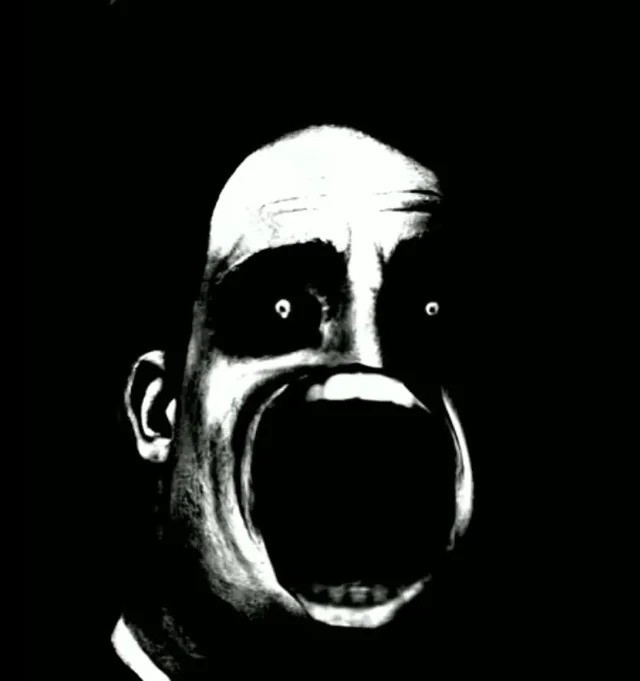
\includegraphics[width=6cm]{uncanny2}
        \captionsetup{labelfont=bf, textfont=it}
        \caption{AHHHH}
        \label{fig:uncanny2}
    \end{figure}
\end{itemize}

\subsection*{Tuesday, 3/12/2024}
\begin{itemize}
    \item See Figure~\ref{fig:uncanny3}.
    \begin{figure}[ht]
        \centering
        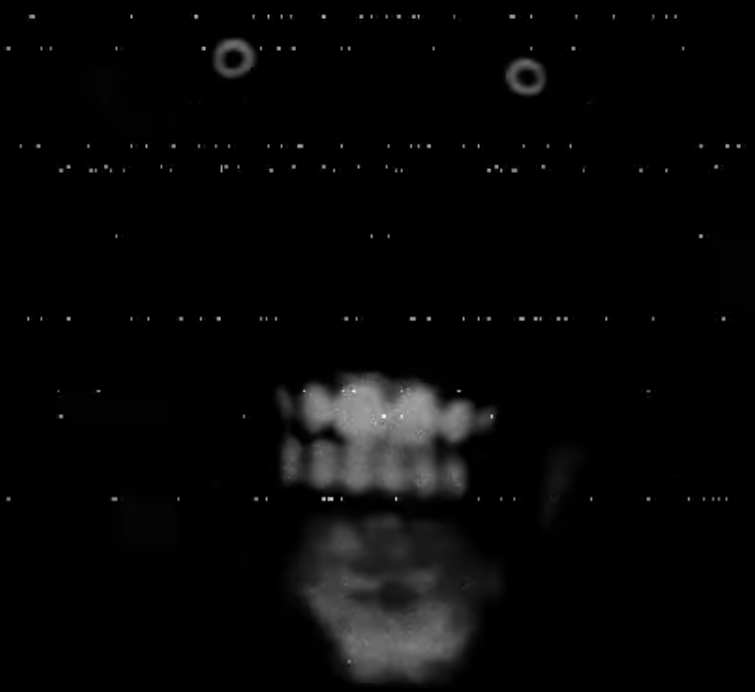
\includegraphics[width=6cm]{uncanny3}
        \captionsetup{labelfont=bf, textfont=it}
        \caption{AHHHHHHHHHHHHHH}
        \label{fig:uncanny3}
    \end{figure}
\end{itemize}

\subsection*{Wednesday, 3/13/2024}
\begin{itemize}
    \item Store articles in local storage to prevent multiple API calls per
        channel per session. Still very clunky behavior with NavBar versus logos
        on ArticleList.
\end{itemize}

\newpage
%%%%%%%%%%%%%%%%%%%%%%%%%%%%%%%%%%%%%%%%%%%%%%%%%%%%%%%%%%%%%%%%%%%%%%%%%%%%%%%
\section{Week 4 SEE WEEK 5}
%%%%%%%%%%%%%%%%%%%%%%%%%%%%%%%%%%%%%%%%%%%%%%%%%%%%%%%%%%%%%%%%%%%%%%%%%%%%%%%

\newpage
%%%%%%%%%%%%%%%%%%%%%%%%%%%%%%%%%%%%%%%%%%%%%%%%%%%%%%%%%%%%%%%%%%%%%%%%%%%%%%%
\section{Week 5}
%%%%%%%%%%%%%%%%%%%%%%%%%%%%%%%%%%%%%%%%%%%%%%%%%%%%%%%%%%%%%%%%%%%%%%%%%%%%%%%
\subsection*{I can't be asked}
\begin{itemize}
    \item I am too lazy to summarize my shitty git commits from the 13 til now
        (the 31st).
    \item Enjoy Mr. Incredible Uncanny 4 instead:
    \begin{figure}[ht]
        \centering
        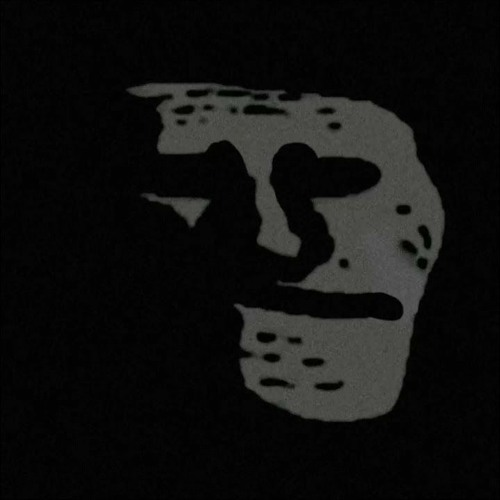
\includegraphics[width=6cm]{uncanny4}
        \captionsetup{labelfont=bf, textfont=it}
        \caption{oooooooooooooooooooo}
        \label{fig:uncanny4}
    \end{figure}
    \item Right, now I've added a few things:
        \begin{itemize}
            \item custom link style and formatting in casts 
            \item render images in casts
            \item sign in with farcaster (doesn't do much else yet)
            \item link to view cast on warpcast 
        \end{itemize}
    \item I suppose I should add reaction data and stuff now.
    \item I'm avoiding the actual hard tech of having the LLM not hallicinate.
        I'm thinking of having a writers room where my proprietary spagetti code
        strips out the things that don't make logical sense from the summary
        from the LLM.
\end{itemize}
\clearpage
\subsection*{I really can't be asked}
\begin{itemize}
    \item I suck at updating this, but I'm focused on a native farcon app at the
        moment. you can check it out
        \textcolor{blue}{\href{https://farcon.info}{here}}.
    \item I'm trying to get messaging working by handcrafting endpoints in rust
        (this will be my downfall, I should just use Neynar) so I'll use them in
        both apps anyways.
    \item Figure~\ref{fig:farcaster_auth} is a drawing (from farcaster YT 
        tutorial) which shows how to create a message with a custom client 
        application.
        \begin{figure}[ht]
            \centering
            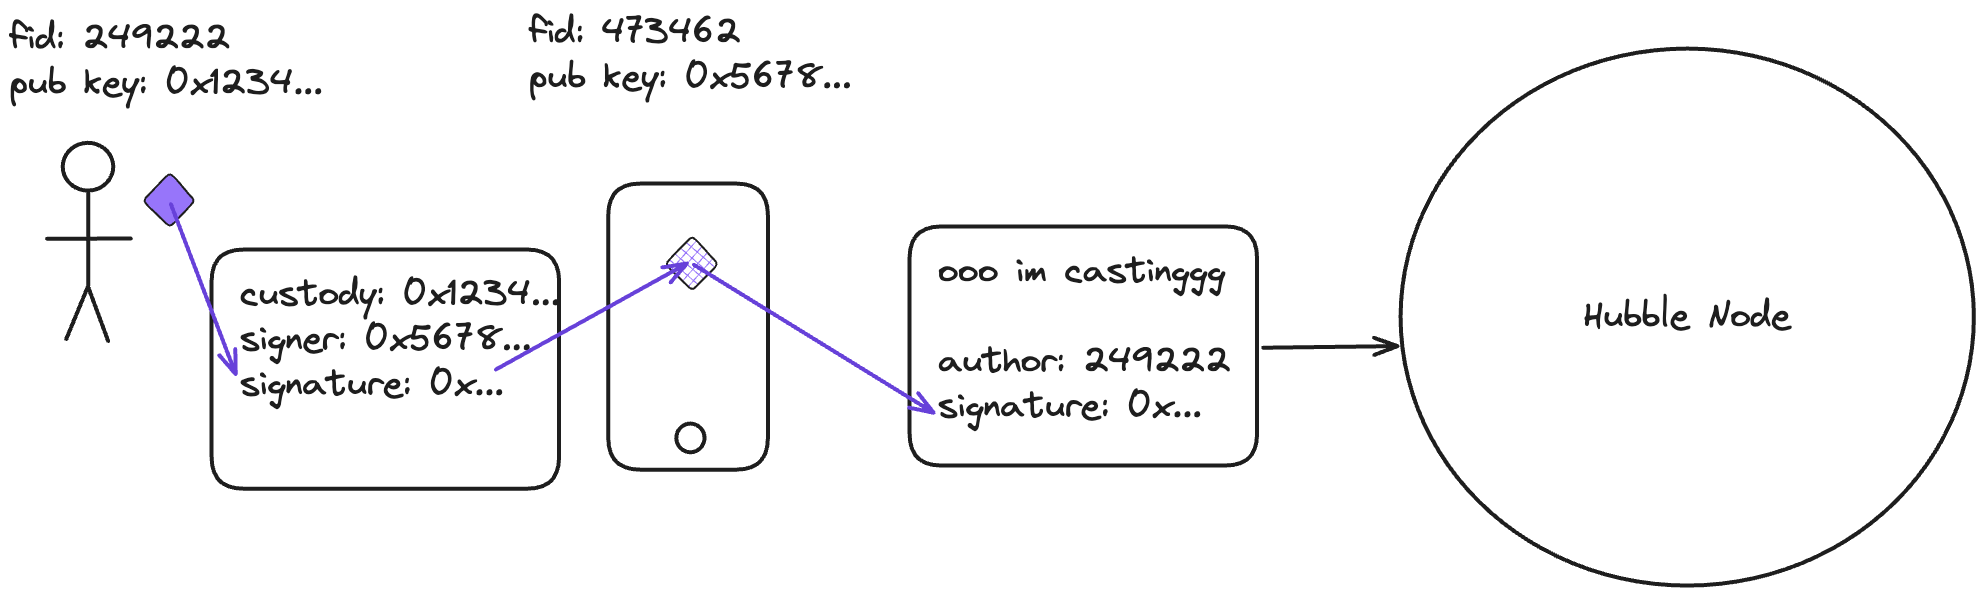
\includegraphics[width=15cm]{farcaster_auth}
            \captionsetup{labelfont=bf, textfont=it}
            \caption{Farcaster Signer Concept}
            \label{fig:farcaster_auth}
        \end{figure}
    \item pinata, farcasterindex, things to thing about using recommended by a
        friend.
\end{itemize}

\newpage
%%%%%%%%%%%%%%%%%%%%%%%%%%%%%%%%%%%%%%%%%%%%%%%%%%%%%%%%%%%%%%%%%%%%%%%%%%%%%%%
\section{Week 7?}
%%%%%%%%%%%%%%%%%%%%%%%%%%%%%%%%%%%%%%%%%%%%%%%%%%%%%%%%%%%%%%%%%%%%%%%%%%%%%%%
\subsection*{04/20/2024}
\subsection*{Saturday, 04/20/2024}
\begin{itemize}
    \item \textcolor{blue}{\href{https://github.com/queazyg}{Q}} is helping me with ai nyt server.
    \item I am hard stuck on messages so perhaps we will crack it together.
\end{itemize}

\subsection*{Sunday, 04/21/2024}
\begin{itemize}
    \item Got diesel initialized in the project for storing articles, have not
        yet tested the ORM yet, I'll do this soon. 
    \item I was distracted by the reactions feature for the network times. This
        was really easy to add, and I styled it indigo-300 or something like
        this. I've never seen a social site have this color like, so it's
        interesting at least.
    \item You can't yet press the like, this will work once I finally figure out
        how to make the app a valid signer for users.
    \item I added a profile page as shown in Figure~\ref{fig:pfp_page}.
        \begin{figure}[ht]
            \centering
            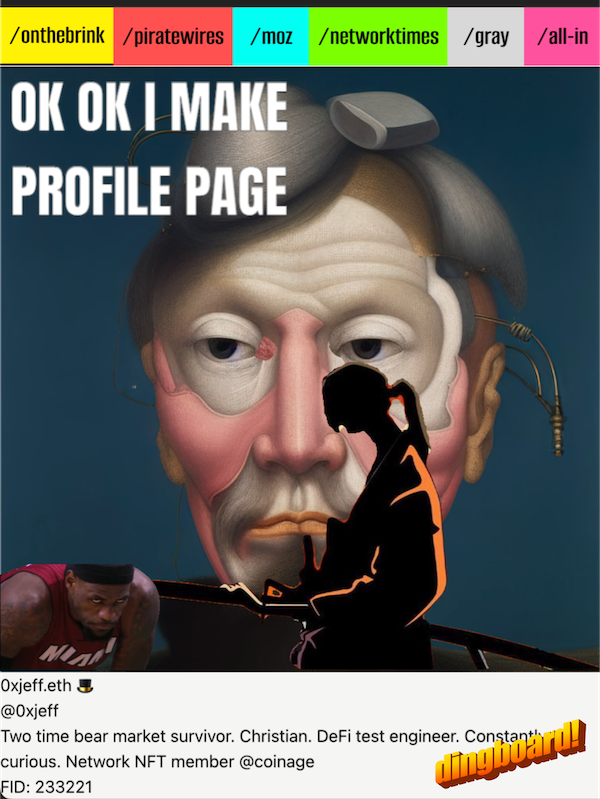
\includegraphics[width=7cm]{pfp_page}
            \captionsetup{labelfont=bf, textfont=it}
            \caption{Profile Page}
            \label{fig:pfp_page}
        \end{figure}
    \item I added hover effects (you can't see it here but matt's pfp background
        has a slight black circle with 10\% opacity applied here
        (Figure~\ref{fig:hover_pfp}).
        \begin{figure}[ht]
            \centering
            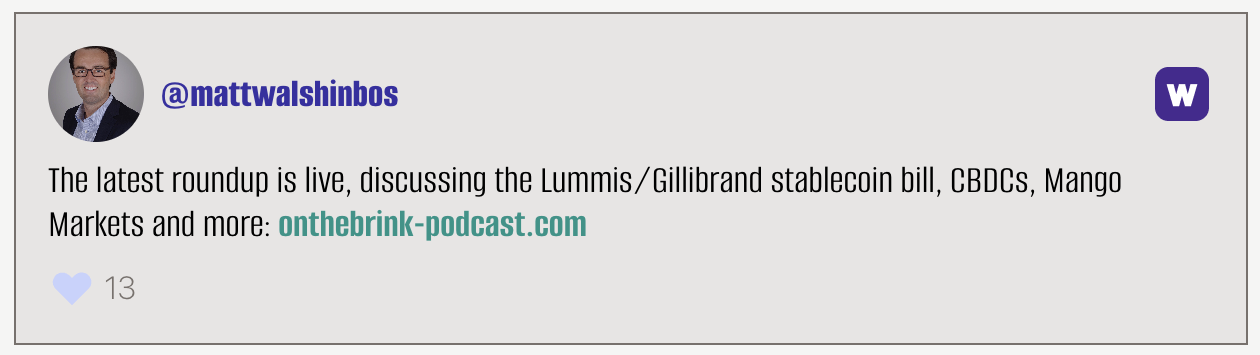
\includegraphics[width=9cm]{hover_pfp}
            \captionsetup{labelfont=bf, textfont=it}
            \caption{Pfp Hover Effect}
            \label{fig:hover_pfp}
        \end{figure}
        \newpage
    \item Distracted once again with iOS app... (Figure~\ref{fig:ios_app_cat})
        \begin{figure}[ht]
            \centering
            
\includegraphics[width=6cm]{ios_app_cat}
            \captionsetup{labelfont=bf, textfont=it}
            \caption{iOS App Cat}
            \label{fig:ios_app_cat}
        \end{figure}
\end{itemize}

\newpage
%%%%%%%%%%%%%%%%%%%%%%%%%%%%%%%%%%%%%%%%%%%%%%%%%%%%%%%%%%%%%%%%%%%%%%%%%%%%%%%
\section{Week 8?}
%%%%%%%%%%%%%%%%%%%%%%%%%%%%%%%%%%%%%%%%%%%%%%%%%%%%%%%%%%%%%%%%%%%%%%%%%%%%%%%
\subsection*{Sunday, 06/10/2024}
\begin{itemize}
    \item we might be back (leptos rewrite). notes from testing existing hubble
        node routes with leptos components.
    \item this is not live yet since it has very limited funtionality.
    \item \texttt{fetch_username} checks if \texttt{lead_usernames} already 
        has the \texttt{fid}. if not, it fetches the username and updates the 
        state.
    \item added \texttt{ongoing_requests} to track fetches and avoid multiple 
        requests for the same \texttt{fid}.
    \item Used \texttt{create_effect} to manage side effects, ensuring 
        usernames are fetched only once.
    \item Used \texttt{spawn_local} for async tasks to keep the main thread 
        non-blocking.
    \item \texttt{Signal} and \texttt{set_signal} handle reactive state in the 
        \texttt{Channels} component, making sure the UI updates when data 
        changes.
    \item \texttt{HashSet} tracks \texttt{ongoing_requests}, preventing 
        duplicate fetches and redundant state updates.
    \item The component dynamically displays usernames from the updated state.
    \item asdfasdf
\end{itemize}

\subsection*{Monday, 06/11/2024}
\begin{itemize}
    \item removed the \texttt{lead_username} variable and its assignment using 
        \texttt{unwrap_or_else} from the \texttt{view!} macro.
    \item added closure inside the \texttt{view!} macrothat matches on 
        \texttt{lead_usernames.get().get(&fid)}.
    \item if the lead username is available show it, else show "chill" in div
        where username would be 
    \item closure is defined using \texttt{move ||} to capture the 
        \texttt{lead_usernames} and \texttt{fid} variables.
\end{itemize}

\subsection*{Tuesday, 06/12/2024}
\begin{itemize}
    \item begin rewrite of cast and cast list pages, need to think about using 
        \texttt{create_effect} in the complicated way that i did above.
    \item using this \texttt{create_effect} in the way that i am to sync the
        reactive system is \textit{officially} discouraged since you might shoot
        off your foot with an infinite loop if you don't create something to
        keep track of the ongoing_requests. i liike the chill message though and
        how it could show up at different times for different channels in some
        cases (probably won't be used, but we will see).
    \item i'll do the cast stuff without \texttt{create_effect} to see
        if it's less complicated and achieves virtually the same thing. 
\end{itemize}


\clearpage
\addcontentsline{toc}{section}{References}
\bibliography{chapters/references} 
\label{sec:references}

\end{document}
